\documentclass[tikz,border=3mm]{standalone}
\usetikzlibrary{matrix, positioning, backgrounds}

\begin{document}
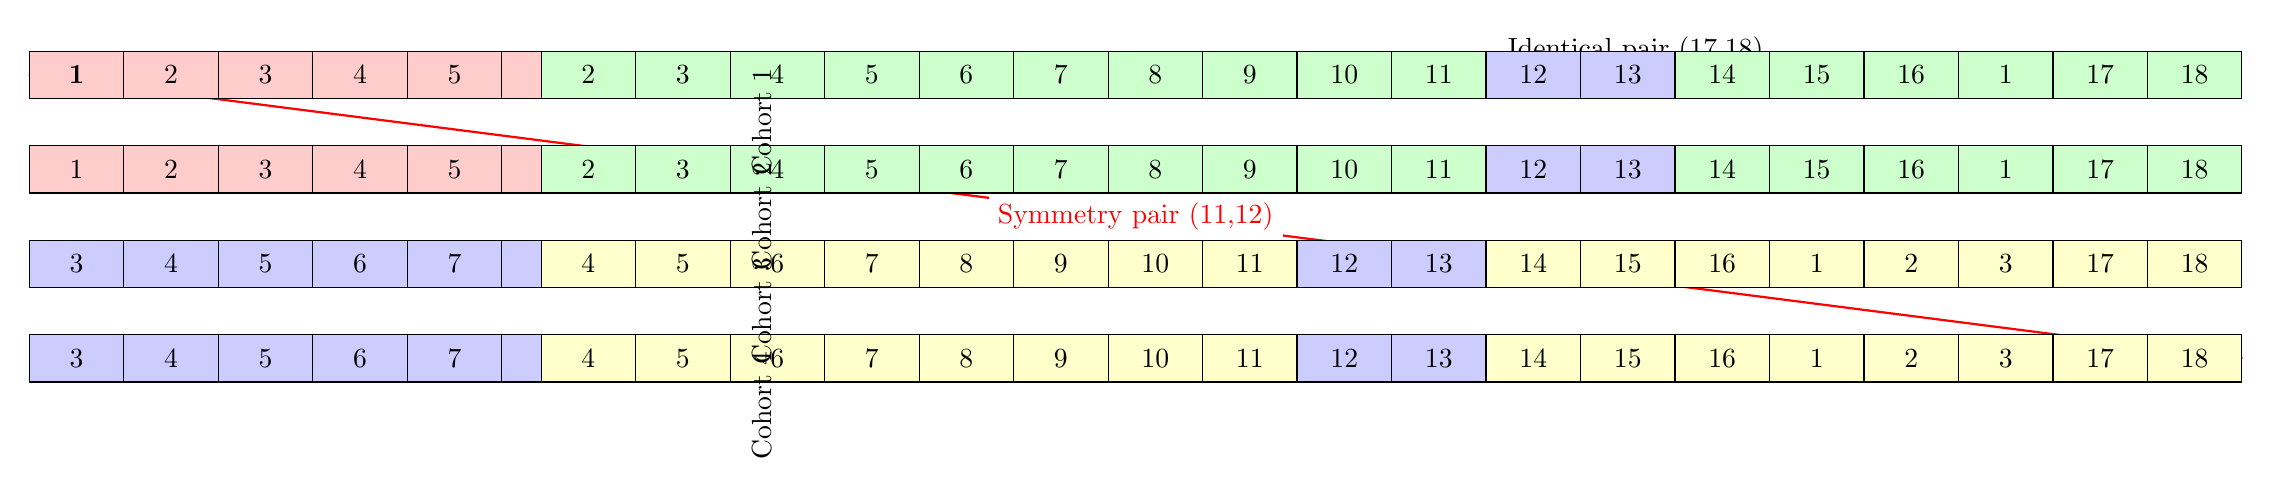
\begin{tikzpicture}[
    agent/.style={
        matrix of nodes,
        nodes={draw, minimum width=1.2cm, minimum height=0.6cm, anchor=center},
        column sep=-\pgflinewidth,
        row sep=-\pgflinewidth,
        inner sep=0pt
    },
    highlight/.style={fill=yellow!30},
    symmetry/.style={fill=blue!20},
    top/.style={font=\bfseries}
]

% Define color scheme
\definecolor{cohort1}{RGB}{255,204,204}
\definecolor{cohort2}{RGB}{204,255,204}
\definecolor{cohort3}{RGB}{204,204,255}
\definecolor{cohort4}{RGB}{255,255,204}

% Cohort 1: Top-left pair
\matrix (A1) at (0,0) [agent, fill=cohort1] {
    |[top]|1 & 2 & 3 & 4 & 5 & 6 & 7 & 8 & 9 & 10 & |[symmetry]|11 & |[symmetry]|12 & 13 & 14 & 15 & 16 & 17 & 18 \\
};
\matrix (A2) at (0,-1.2) [agent, fill=cohort1] {
    1 & 2 & 3 & 4 & 5 & 6 & 7 & 8 & 9 & 10 & |[symmetry]|11 & |[symmetry]|12 & 13 & 14 & 15 & 16 & 17 & 18 \\
};

% Cohort 2: Top-right pair
\matrix (B1) at (6.5,0) [agent, fill=cohort2] {
    2 & 3 & 4 & 5 & 6 & 7 & 8 & 9 & 10 & 11 & |[symmetry]|12 & |[symmetry]|13 & 14 & 15 & 16 & 1 & 17 & 18 \\
};
\matrix (B2) at (6.5,-1.2) [agent, fill=cohort2] {
    2 & 3 & 4 & 5 & 6 & 7 & 8 & 9 & 10 & 11 & |[symmetry]|12 & |[symmetry]|13 & 14 & 15 & 16 & 1 & 17 & 18 \\
};

% Cohort 3: Bottom-left pair
\matrix (C1) at (0,-2.4) [agent, fill=cohort3] {
    3 & 4 & 5 & 6 & 7 & 8 & 9 & 10 & 11 & |[symmetry]|12 & |[symmetry]|13 & 14 & 15 & 16 & 1 & 2 & 17 & 18 \\
};
\matrix (C2) at (0,-3.6) [agent, fill=cohort3] {
    3 & 4 & 5 & 6 & 7 & 8 & 9 & 10 & 11 & |[symmetry]|12 & |[symmetry]|13 & 14 & 15 & 16 & 1 & 2 & 17 & 18 \\
};

% Cohort 4: Bottom-right pair
\matrix (D1) at (6.5,-2.4) [agent, fill=cohort4] {
    4 & 5 & 6 & 7 & 8 & 9 & 10 & 11 & |[symmetry]|12 & |[symmetry]|13 & 14 & 15 & 16 & 1 & 2 & 3 & 17 & 18 \\
};
\matrix (D2) at (6.5,-3.6) [agent, fill=cohort4] {
    4 & 5 & 6 & 7 & 8 & 9 & 10 & 11 & |[symmetry]|12 & |[symmetry]|13 & 14 & 15 & 16 & 1 & 2 & 3 & 17 & 18 \\
};

% Labels
\foreach \i in {1,...,4} {
    \node at (-1.5, -\i*1.2 + 0.6) {\rotatebox{90}{Cohort \i}};
}

% Annotations
\begin{scope}[on background layer]
    \draw[thick, red] (A1-1-1.west) -- (D2-1-18.east) 
        node[midway, fill=white] {Symmetry pair (11,12)};
    \draw[thick, green!60!black] (A1-1-17.west) -- (A1-1-18.east)
        node[midway, above, black] {Identical pair (17,18)};
    \foreach \m in {A1,A2,B1,B2,C1,C2,D1,D2} {
        \draw[thick, green!60!black] (\m-1-17.west) -- (\m-1-18.east);
    }
\end{scope}

\end{tikzpicture}
\end{document}